\section{Spring MVC}
Nello sviluppo di una API REST tramite Spring Boot è comune l'utilizzo del pattern architetturale Model-View-Controller(MVC).\\

\begin{figure}[H] 
    \centering 
    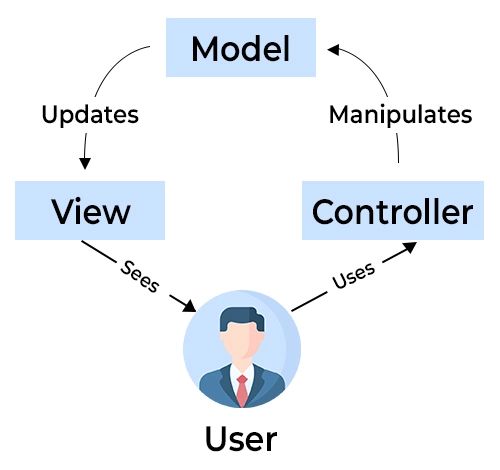
\includegraphics[width=0.50\columnwidth]{mvc2} 
    \caption{Schema Model-View-Controller}
\end{figure}

\subsection{Model}
Il Modello o Model in inglese, rappresenta i dati e i metodi per accedere ai dati dell'applicazione. Se esso viene aggiornato in seguito ad azioni o eventi, notificherà la View e il Controller del cambiamento.\\
Nel contesto dello sviluppo di un'API REST, il Model contiene dati che vengono elaborati e restituiti dall'API.\\
All'interno del progetto il Model è formato dai seguenti elementi.
\subsubsection*{Entità}
Le entità sono risorse rappresentate con classi Java segnate a class level\textsubscript{g} con l'annotazione\textsubscript{g} \textit{@Entity}. Questa annotazione viene utilizzata per identificare una classe che è mappata\textsubscript{g} su una tabella nel database. All'interno di queste classi, vengono dichiarati gli attributi corrispondenti alla tabella di riferimento utilizzando annotazioni JPA appropriate, e vengono gestite le relazioni tra le tabelle attraverso altre annotazioni.
\subsubsection*{Repository}
Le repository implementate nel progetto gestiscono l'accesso ai dati e definiscono metodi per eseguire operazioni di base sui dati, come l'inserimento, la modifica, la cancellazione e la ricerca. Tutto questo è stato possibile all'interno del progetto estendendo interfacce JPA, che consentono di eseguire operazioni in una base di dati senza scrivere codice SQL.
\subsubsection*{DTO}
Data Transfer Object (DTO), oggetti utilizzati per modellare le rappresentazioni dei dati, utilizzati per definire sia i dati inviati dal client nelle richieste che quelli che inviati dal server al cliente nelle risposte.\\

\subsection{View}
La Vista o View in inglese, è responsabile di mostrare i dati provenienti dal Model e dell'interazione con l'utente. Essa cattura gli input dell'utente e delega al Controller l'elaborazione.\\
Dato che il progetto si concentrava sul lato back-end, precisamente sullo sviluppo dell'API REST, non ho quindi sviluppato una vera e propria View, poichè l'output è in formato JSON. In questo contesto l'output prodotto contenente i dati presentati al client in formato JSON, potrebbe essere considerata come "View".\\

\subsection{Controller}
Il Controller gestisce il flusso dell'applicazione. Esso riceve i comandi dell'utente attraverso la View e reagisce eseguendo operazioni conseguenti. Queste sue operazioni possono o meno coinvolgere il Model, ma portano generalmente sempre ad un cambiamento di stato della View.\\
All'interno del meccanismo di Spring MVC il Controller gestisce le richieste HTTP in arrivo, selezionando il Controller adeguato. Sono quindi responsabili di ricevere le richieste, elaborarle e restituire le risposte corrispondenti.\\
All'interno del progetto il Controller è formato dai seguenti elementi.
\subsubsection*{Controller}
I Controller contengono i metodi a cui vengono associati i percorsi delle richieste HTTP. Esso interpreta i parametri che possono provenire dall'URL o dal corpo della richiesta. Internamente a questi metodi viene richiamato il Service appropriato per eseguire operazioni di business logic al risultato finale da restituire.\\
Per garantire che i dati inseriti dagli utenti o provenienti da richieste siano conformi alle aspettative e non causino errori vengono inseriti dei controlli di validazioni all'interno dei metodi del Controller.
\subsubsection*{Service}
I Service eseguono operazioni complesse ed elaborazioni di dati, gestendo la business logic dell'applicazione. Essi interagiscono con i Repository per recuperare dati dal database e vengono richiamati all'interno dei metodi del Controller. Contengono ulteriori controlli di validazione per verificare la correttezza dei dati utilizzati.
\subsubsection*{Exception Handler}
Per centralizzare la gestione delle eccezioni è stato creato un handler che garantisce uniformità alle eccezioni che l'applicazione può produrre.\\
